% !TEX encoding = UTF-8
\documentclass[12pt,a4paper]{article}

% Vietnamese support
\usepackage[utf8]{inputenc}
\usepackage[vietnamese]{babel}
\usepackage{amsmath,amssymb}
\usepackage{graphicx}
\usepackage{float}
\usepackage{booktabs}
\usepackage{tabularx}
\usepackage{geometry}
\usepackage{caption}
\usepackage{subcaption}
\usepackage{hyperref}
\usepackage{listings}
\usepackage{xcolor}
\usepackage{fancyhdr}
\usepackage{titlesec}
\usepackage{enumitem}
\usepackage{multirow}
\usepackage{array}
\usepackage{longtable}

\geometry{left=2.5cm, right=2cm, top=2.5cm, bottom=2.5cm}
\setlength{\headheight}{13.75pt}
\addtolength{\topmargin}{-1.6pt}

% Code listing style
\lstset{
    language=Tcl,
    basicstyle=\ttfamily\small,
    keywordstyle=\color{blue}\bfseries,
    commentstyle=\color{gray}\itshape,
    stringstyle=\color{red},
    numbers=left,
    numberstyle=\tiny\color{gray},
    numbersep=5pt,
    breaklines=true,
    frame=single,
    rulecolor=\color{black!30},
    backgroundcolor=\color{gray!5},
    showstringspaces=false,
    tabsize=4,
    captionpos=b
}

% Header/Footer
\pagestyle{fancy}
\fancyhf{}
\fancyhead[L]{\small Báo Cáo Thiết Kế Vật Lý -- Innovus}
\fancyhead[R]{\small \thepage}

% Bullet style: use dashes
\setlist[itemize]{label={--}}

% Title format
\titleformat{\section}{\Large\bfseries}{\thesection.}{0.5em}{}
\titleformat{\subsection}{\large\bfseries}{\thesubsection.}{0.5em}{}
\titleformat{\subsubsection}{\normalsize\bfseries}{\thesubsubsection.}{0.5em}{}

\begin{document}

%====================================================================
% TITLE PAGE
%====================================================================
\begin{titlepage}
\centering
\vspace*{2cm}
{\Huge\bfseries Báo Cáo Thiết Kế Vật Lý\\[0.3cm]}
{\Huge\bfseries Flow Innovus - Dự Án Môn Học\\[0.5cm]}
{\Large Khối thiết kế: \texttt{croc\_chip}}\\[1cm]

\vspace{1cm}
{\large
\begin{tabular}{ll}
\textbf{Công nghệ:} & IHP SG13G2 (130nm) \\
\textbf{Tần số mục tiêu:} & 100 MHz (chu kỳ 10,0 ns) \\
\textbf{Clock Uncertainty:} & 0,1 ns \\
\textbf{Công cụ EDA:} & Cadence Innovus \\
\end{tabular}
}

\vspace{2cm}
\vfill
\end{titlepage}

\tableofcontents
\newpage

%====================================================================
% 1. TỔNG QUAN VÀ SETUP
%====================================================================
\section{Tổng Quan và Setup Hệ Thống}
Báo cáo này trình bày quy trình thiết kế vật lý (Physical Design - PD) cho khối thiết kế \texttt{croc\_chip} sử dụng công nghệ IHP SG13G2.

Các ràng buộc về timing được định nghĩa trong file \texttt{constraints.sdc}, trong đó tần số mục tiêu là 100MHz (chu kỳ $T = 10,0$ ns), được thiết lập cùng với độ trễ Uncertainty (cả setup và hold) là 0,1 ns.

\begin{lstlisting}[caption={Quy định timing constraint}]
set TCK_SYS 10.0
create_clock -name clk_sys -period $TCK_SYS [get_ports clk_i]

set_clock_uncertainty 0.1 -setup [all_clocks]
set_clock_uncertainty 0.1 -hold [all_clocks]
set_clock_transition  0.2 [all_clocks]
\end{lstlisting}

%====================================================================
% 2. FLOORPLANNING
%====================================================================
\section{Floorplanning (00 \& 01)}

\subsection{Kích thước Core và Die}
Giai đoạn Floorplan khởi tạo kích thước die và core của chip, thiết lập các vùng để đặt standard cells. Chiều dài viền biên (margin) từ lõi (core) đến cạnh die được thiết lập là 168 $\mu$m ở cả 4 cạnh để chừa không gian cho I/O rings hoặc pad.

\begin{lstlisting}[caption={Khởi tạo Floorplan}]
floorPlan -site CoreSite -d 1840.32 1840.02 168 168 168 168
\end{lstlisting}

\begin{itemize}
    \item \textbf{Die Area:} 1840,32 $\times$ 1840,02 $\mu$m
    \item \textbf{Core Area:} Được tính toán tự động dựa trên margin 168 $\mu$m ở các cạnh.
    \item \textbf{Utilization mục tiêu:} Khoảng 58\%.
\end{itemize}

\subsection{Thông số Routing Layer}
Thiết kế sử dụng các lớp kim loại (Metal layers) được quy định trong tập tin LEF. Bảng dưới đây mô tả thông số chiều rộng (width), khoảng cách (spacing) và bước (pitch) của 7 lớp metal cơ bản được sử dụng trong việc routing cũng như thiết kế lưới nguồn (Power Grid).

\begin{table}[H]
    \centering
    \caption{Thông số Metal Layer theo file LEF}
    \label{tab:metal_rules}
    \begin{tabular}{|l|c|c|c|c|}
        \hline
        \textbf{Layer} & \textbf{Hướng (Direction)} & \textbf{Pitch ($\mu$m)} & \textbf{Width ($\mu$m)} & \textbf{Spacing ($\mu$m)} \\
        \hline
        Metal1 & Vertical & 0,48 & 0,16 & 0,18 \\
        Metal2 & Horizontal & 0,42 & 0,20 & 0,22 \\
        Metal3 & Vertical & 0,48 & 0,20 & 0,22 \\
        Metal4 & Horizontal & 0,42 & 0,20 & 0,22 \\
        Metal5 & Vertical & 0,48 & 0,20 & 0,42 \\
        TopMetal1 & Horizontal & 2,28 & 1,64 & 1,64 \\
        TopMetal2 & Vertical & 4,00 & 2,00 & 2,00 \\
        \hline
    \end{tabular}
\end{table}

\subsection{Mạng lưới nguồn PG Mesh}
Lưới nguồn và đất (Power/Ground Mesh) được tạo trên các lớp cao để phân phối điện năng ổn định. PG Mesh được thiết kế với VDD và VSS chạy qua M3, M4, M5, TopMetal1, và TopMetal2. Bảng dưới đây mô tả chi tiết thông số bề rộng (width), khoảng cách set-to-set và khoảng cách (spacing) cho từng lớp Metal:

\begin{table}[H]
    \centering
    \caption{Thông số lưới nguồn PG Mesh}
    \begin{tabular}{|l|c|c|c|c|}
        \hline
        \textbf{Layer} & \textbf{Hướng} & \textbf{Width ($\mu$m)} & \textbf{Set-to-set ($\mu$m)} & \textbf{Spacing ($\mu$m)} \\
        \hline
        Metal3 & Vertical & 1 & 15 & 2 \\
        Metal4 & Horizontal & 1 & 15 & 2 \\
        Metal5 & Vertical & 1 & 15 & 2 \\
        TopMetal1 & Horizontal & 4 & 30 & 4 \\
        TopMetal2 & Vertical & 4 & 30 & 4 \\
        \hline
    \end{tabular}
\end{table}

Các lệnh \texttt{addstripe} cấu hình độ dày, hướng, khoảng cách, và via kết nối giữa các lớp.

\begin{lstlisting}[caption={Cấu trúc PG Mesh}]
# Metal3 (Vertical)
setAddStripeMode -reset
setAddStripeMode -stacked_via_top_layer Metal3 -stacked_via_bottom_layer Metal1 -stapling_nets_style side_to_side
addstripe -layer Metal3 -direction vertical -nets {VDD VSS} -width 1 -set_to_set_distance 15 -spacing 2 -start 0.5

# Metal4 (Horizontal)
setAddStripeMode -reset
setAddStripeMode -stacked_via_top_layer Metal4 -stacked_via_bottom_layer Metal3 -stapling_nets_style side_to_side
addstripe -layer Metal4 -direction horizontal -nets {VDD VSS} -width 1 -set_to_set_distance 15 -spacing 2 -start 0.5

# Metal5 (Vertical)
setAddStripeMode -stacked_via_top_layer Metal5 -stacked_via_bottom_layer Metal4 -stapling_nets_style side_to_side
addstripe -layer Metal5 -direction vertical   -nets {VDD VSS} -width 1 -set_to_set_distance 15 -spacing 2 -start 0.5

# TopMetal1 (Horizontal)
setAddStripeMode -stacked_via_top_layer TopMetal1 -stacked_via_bottom_layer Metal5 -stapling_nets_style side_to_side
addstripe -layer TopMetal1 -direction horizontal -nets {VDD VSS} -width 4 -set_to_set_distance 30 -spacing 4 -start 0.5

# TopMetal2 (Vertical)
setAddStripeMode -stacked_via_top_layer TopMetal2 -stacked_via_bottom_layer TopMetal1 -stapling_nets_style side_to_side
addstripe -layer TopMetal2 -direction vertical   -nets {VDD VSS} -width 4 -set_to_set_distance 30 -spacing 4
\end{lstlisting}

\begin{figure}[H]
    \centering
    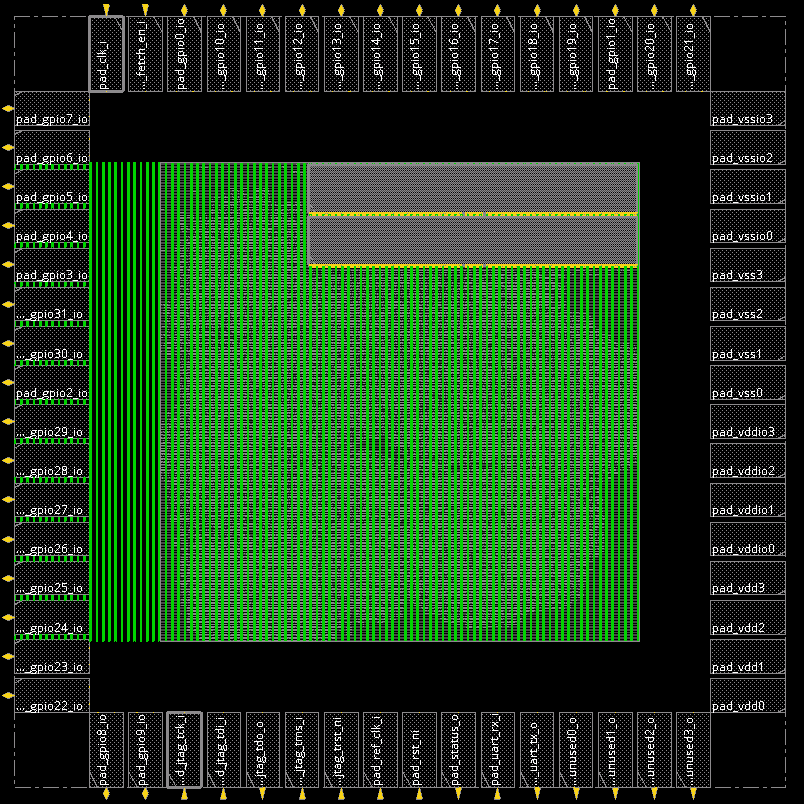
\includegraphics[width=0.45\textwidth]{pgmesh_metal3.png}
    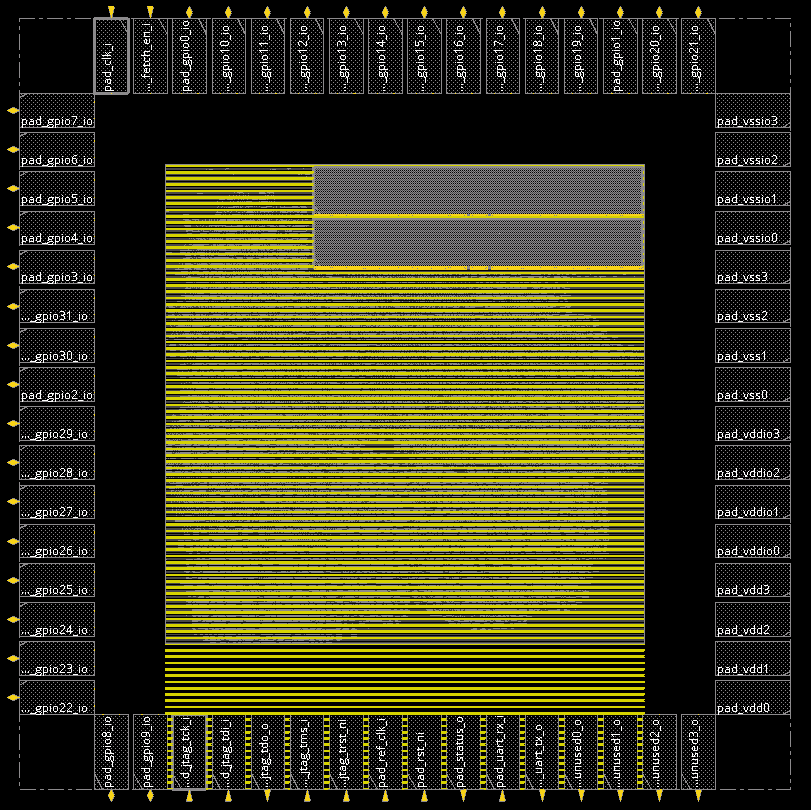
\includegraphics[width=0.45\textwidth]{pgmesh_metal4.png}
    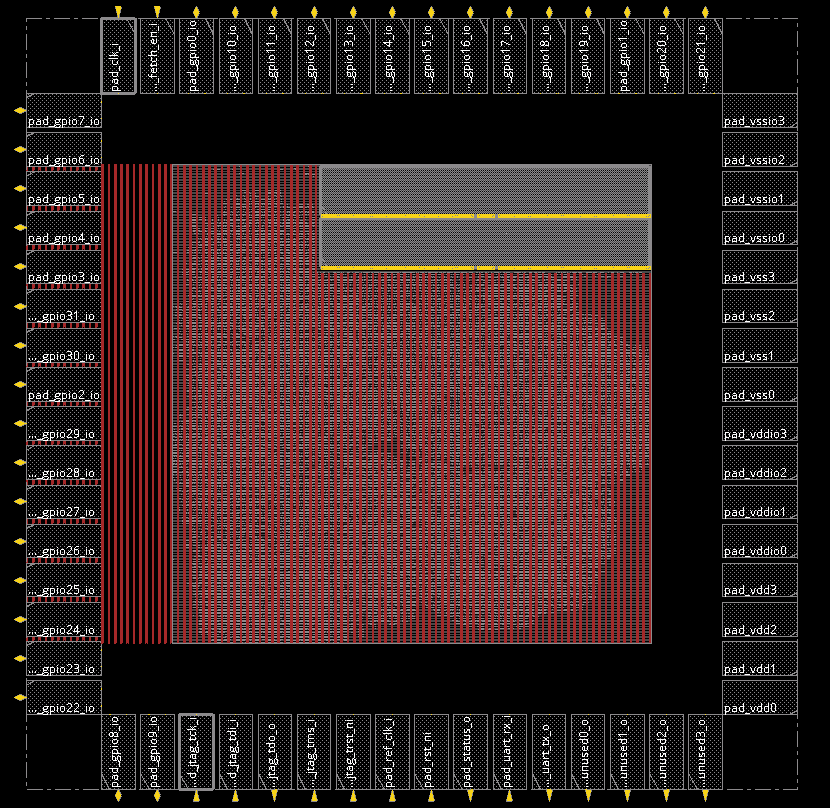
\includegraphics[width=0.45\textwidth]{pgmesh_metal5.png}
    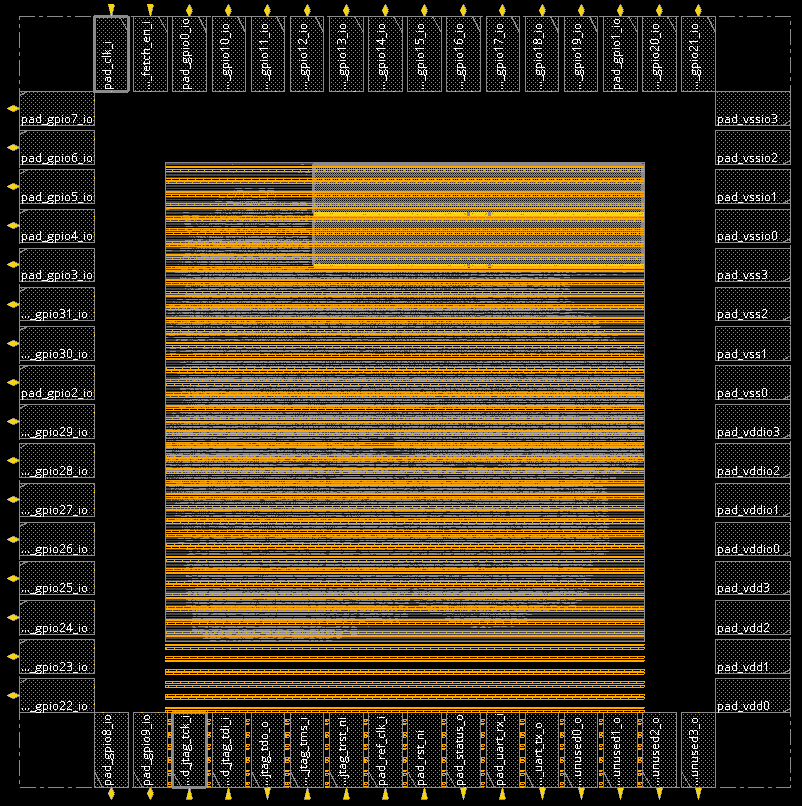
\includegraphics[width=0.45\textwidth]{pgmesh_topmetal1.png}
    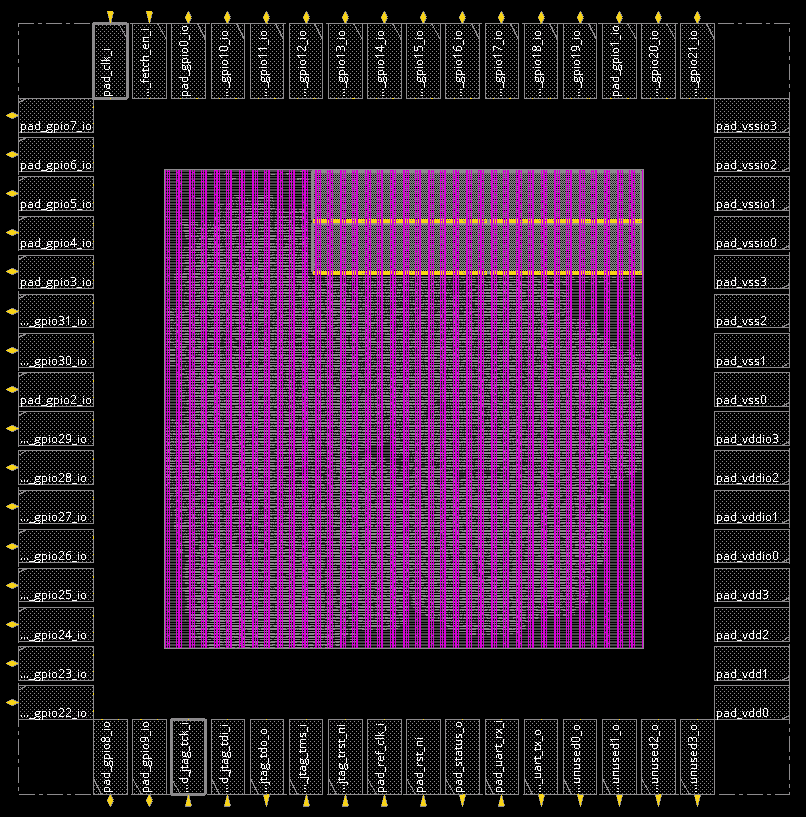
\includegraphics[width=0.45\textwidth]{pgmesh_topmetal2.png}
    \caption{Lưới PG Mesh ở các tầng (M3, M4, M5, TM1, TM2)}
\end{figure}

\begin{figure}[H]
    \centering
    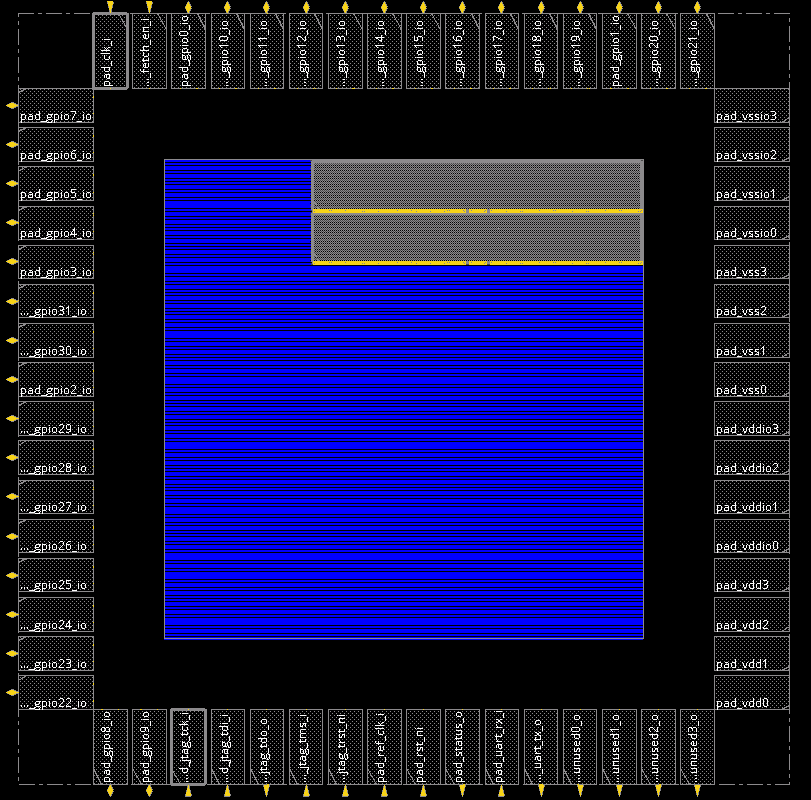
\includegraphics[width=0.45\textwidth]{pgmesh_metal1_rail.png}
    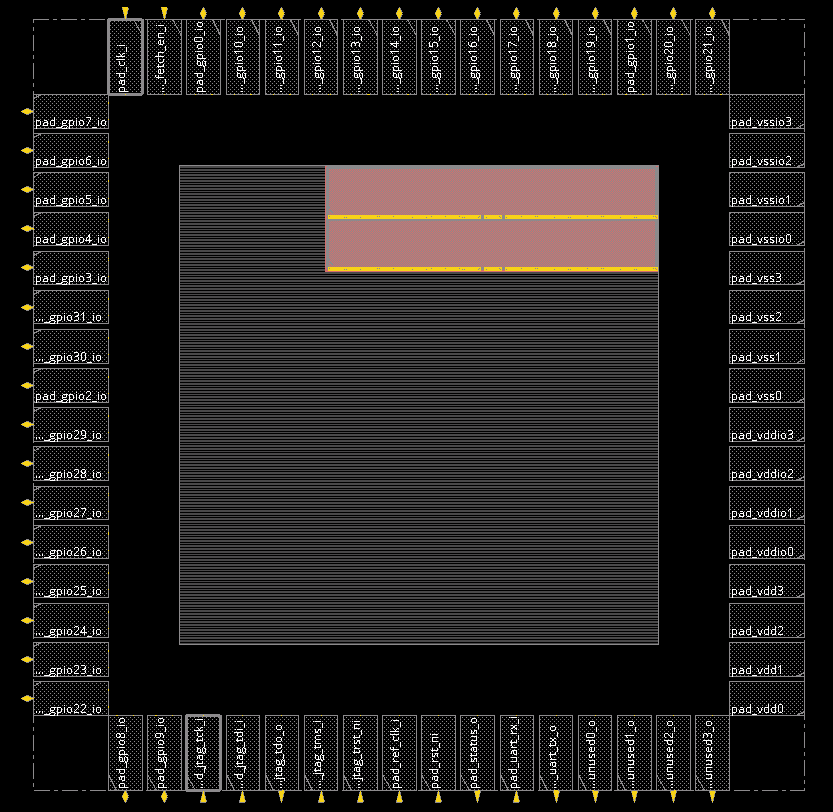
\includegraphics[width=0.45\textwidth]{00_init+floorplan.png}
    \caption{Power rails M1 (trái) và Floorplan hoàn chỉnh (phải)}
\end{figure}

%====================================================================
% 3. PLACEMENT
%====================================================================
\section{Placement (02)}

Quá trình Placement thực thi bước sắp xếp các standard cells và cell nội bộ vào đúng hàng (row). Các block logic thao tác trực tiếp với bộ nhớ SRAM được yêu cầu đặt sát các viền SRAM để tối ưu routing và giảm độ trễ (wirelength).

\begin{lstlisting}[caption={Lệnh Placement và tạo Tie Cells}]
place_opt_design

setTieHiLoMode -reset
setTieHiLoMode -cell {sg13g2_tiehi sg13g2_tielo} -maxFanOut 10
addTieHiLo -cell {sg13g2_tiehi sg13g2_tielo} -prefix TIE
\end{lstlisting}

\subsection{Bố cục SRAM và Block Logic}
Dưới đây là sơ đồ hiển thị các block logic (điểm màu) được phân bổ tối ưu để nằm cạnh các khối SRAM tương ứng. Khối SRAM cũng được trang bị các blockages xung quanh thân (Halo).

\begin{figure}[H]
    \centering
    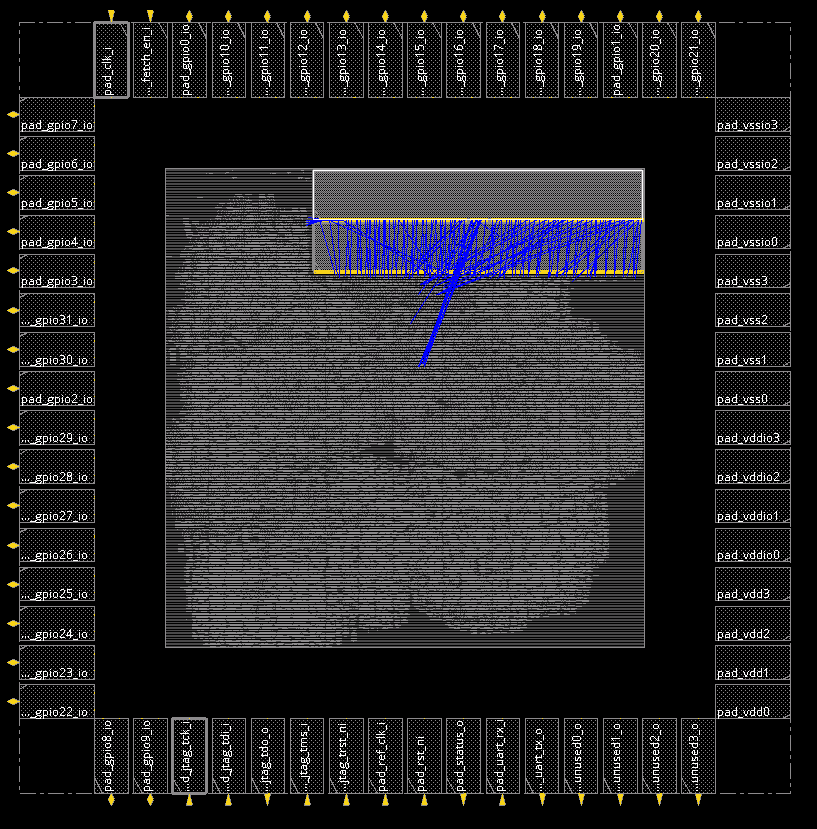
\includegraphics[width=0.45\textwidth]{sram_nearly_std_same_logic_1.png}
    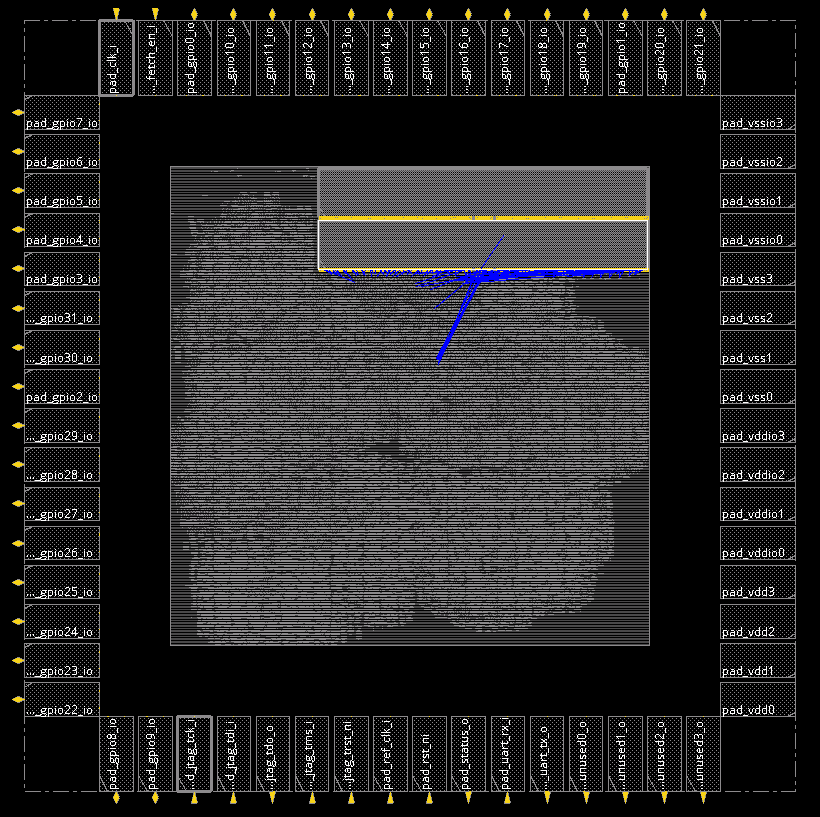
\includegraphics[width=0.45\textwidth]{sram_nearly_std_same_logic_2.png}
    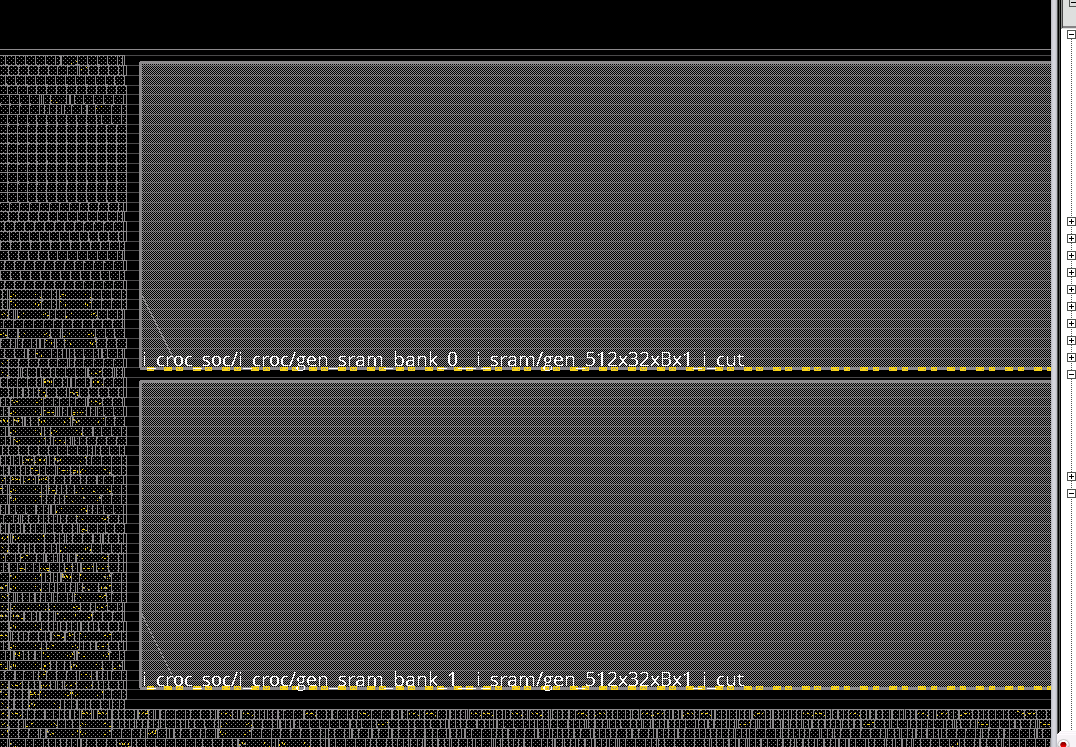
\includegraphics[width=0.45\textwidth]{sram_place_halo.png}
    \caption{SRAM placement, logic liền kề, và khoảng cách Halo}
\end{figure}

\subsection{Hiệu chỉnh Redundant Buffer bằng dòng lệnh (ECO)}
Sau khi placement hoàn tất, timing report cho thấy xuất hiện 9 redundant buffers gây ảnh hưởng tiêu cực lên critical paths (path bị lỗi timing). Lỗi này được sửa thủ công ở chế độ ECO (Engineering Change Order) bằng cách gỡ bỏ buffer dư thừa.

\begin{lstlisting}[caption={Xóa redundant buffers (ECO script)}]
setEcoMode -batchMode true
ecoDeleteRepeater -inst <ten_instance_buffer_1>
ecoDeleteRepeater -inst <ten_instance_buffer_2>
# ... lap lai de go bo toan bo 9 buffer du thua ...
setEcoMode -batchMode false
\end{lstlisting}

\begin{figure}[H]
    \centering
    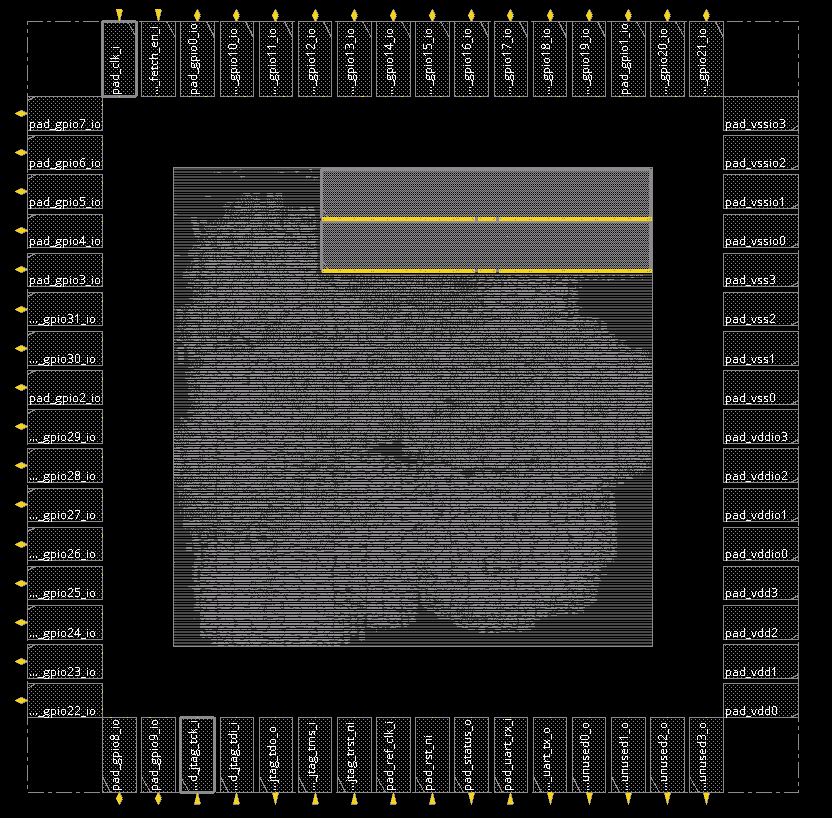
\includegraphics[width=0.7\textwidth]{02_placement.png}
    \caption{Bản đồ chip sau khi hoàn tất Placement}
\end{figure}

\subsection{Timing Report (Post-Placement)}
Bảng dưới đây trình bày timing tổng quan sau khi placement (chỉ tính timing nội bộ). Các đường truyền với I/O ports bị bỏ qua. Ở giai đoạn này, reg2reg WNS bị âm nhẹ (-0,033 ns).

\begin{table}[H]
    \centering
    \caption{Timing nội bộ sau Placement}
    \begin{tabular}{|l|c|c|c|}
        \hline
        \textbf{Loại (Path Type)} & \textbf{WNS (ns)} & \textbf{TNS (ns)} & \textbf{Đường vi phạm (Vio)} \\
        \hline
        \textbf{reg $\rightarrow$ reg} & -0,033 & -0,366 & 33 \\
        \textbf{reg $\rightarrow$ mem} & 0,719 & 0,000 & 0 \\
        \textbf{mem $\rightarrow$ reg} & 0,054 & 0,000 & 0 \\
        \hline
    \end{tabular}
\end{table}


%====================================================================
% 4. CLOCK TREE SYNTHESIS
%====================================================================
\section{Clock Tree Synthesis (CTS - 03 \& 04)}

CTS là giai đoạn tổng hợp cây đồng hồ nhằm cung cấp tín hiệu clock cho toàn bộ thanh ghi (registers) trong thiết kế sao cho đồng pha và có độ trễ cân bằng (minimum skew). Lệnh \texttt{optDesign -postCTS} thực hiện tinh chỉnh và tối ưu thiết kế, đưa giá trị timing của \texttt{reg2reg} chuyển sang dương.

\begin{lstlisting}[caption={Thực thi CTS và tối ưu (CTS\_opt)}]
clockDesign -outDir ../rpt/${STAGE}/${STAGE}_clk
optDesign -postCTS
optDesign -postCTS -hold
\end{lstlisting}

\begin{figure}[H]
    \centering
    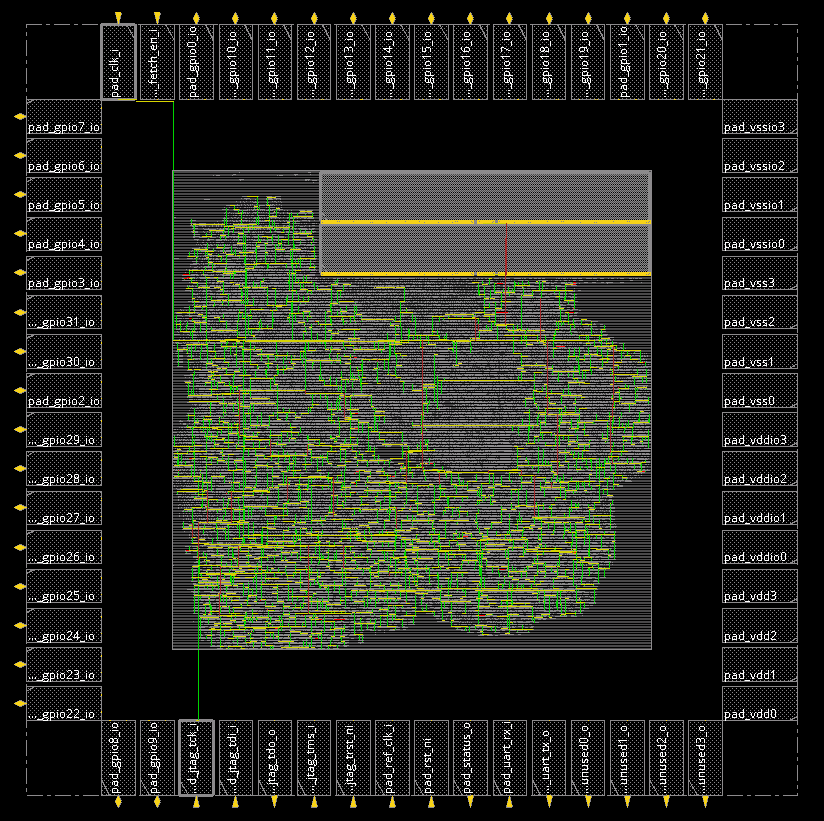
\includegraphics[width=0.7\textwidth]{03_cts.png}
    \caption{Giao diện tuyến đường dây Clock (Clock Tree)}
\end{figure}

\subsection{Timing Report (Post-CTS)}
Kết quả của \texttt{optDesign} sau quá trình CTS chứng minh tính hiệu quả khi không còn đường vi phạm nào ở path \texttt{reg2reg} (WNS dương). Mọi đường vi phạm (WNS = -2,700 ns) còn lại trong Summary tổng thể chỉ đến từ giao tiếp in/out.

\begin{table}[H]
    \centering
    \caption{Timing nội bộ sau CTS}
    \begin{tabular}{|l|c|c|c|}
        \hline
        \textbf{Loại (Path Type)} & \textbf{WNS (ns)} & \textbf{TNS (ns)} & \textbf{Đường vi phạm (Vio)} \\
        \hline
        \textbf{reg $\rightarrow$ reg} & 0,001 & 0,000 & 0 \\
        \textbf{reg $\rightarrow$ mem} & 0,638 & 0,000 & 0 \\
        \textbf{mem $\rightarrow$ reg} & 0,044 & 0,000 & 0 \\
        \hline
    \end{tabular}
\end{table}

%====================================================================
% 5. ROUTING
%====================================================================
\section{Routing (05 \& 06)}

Công cụ NanoRoute của Innovus thực hiện Global Routing và Detailed Routing. Dựa trên file cấu hình \texttt{config.tcl}, tầng kim loại được phép định tuyến (routing layers) được giới hạn từ \texttt{Metal1} lên đến tối đa \texttt{Metal5}. Điều này dành các lớp \texttt{TopMetal1} và \texttt{TopMetal2} hoàn toàn cho mạng lưới phân phối nguồn (PG Mesh).

\begin{lstlisting}[caption={Giới hạn lớp định tuyến}]
setDesignMode -topRoutingLayer Metal5
setDesignMode -bottomRoutingLayer Metal1
\end{lstlisting}

Bên cạnh đó, lệnh khai báo NanoRoute kích hoạt tính năng định tuyến điều hướng theo timing (timing-driven) và ngăn ngừa nhiễu điện từ (si-driven).

\begin{lstlisting}[caption={Cấu hình NanoRoute và tiến hành Routing (05\_route.tcl)}]
setNanoRouteMode -quiet -routeWithTimingDriven 1
setNanoRouteMode -quiet -routeWithSiDriven 1
setNanoRouteMode -routeExpAdvancedPinAccess 2
routeDesign -globalDetail
\end{lstlisting}

\subsection{Tối ưu với Useful Skew}
Để giải quyết những vi phạm timing cuối cùng ở giai đoạn sau khi Route, thuật toán \textbf{Useful Skew} được kích hoạt trong lệnh \texttt{optDesign -postRoute}. Thay vì đảm bảo toàn bộ clock đều đến đích tại cùng một thời điểm, Useful Skew điều chỉnh bộ đệm để các flop điểm cuối nhận clock trễ/sớm hơn nhằm "mượn" thời gian bù trừ cho delay của đường truyền tín hiệu trước nó.

\begin{lstlisting}[caption={Áp dụng Useful Skew trong Post-Route Optimization}]
setOptMode -usefulSkew true
setOptMode -usefulSkewPostRoute true
setOptMode -addInstancePrefix ictc_postRoute_extra_
optDesign -postRoute
optDesign -postRoute -hold
\end{lstlisting}

\subsection{Cấu trúc Metal Layers và Tối ưu Final (Finishing)}
Dưới đây là hình ảnh cắt lớp cho từng Metal layer và hiển thị của cell nối tiếp (Filler cells) để lấp các khoảng trống giữa standard cells (ngừa lỗi DRC về giếng điện).

\begin{figure}[H]
    \centering
    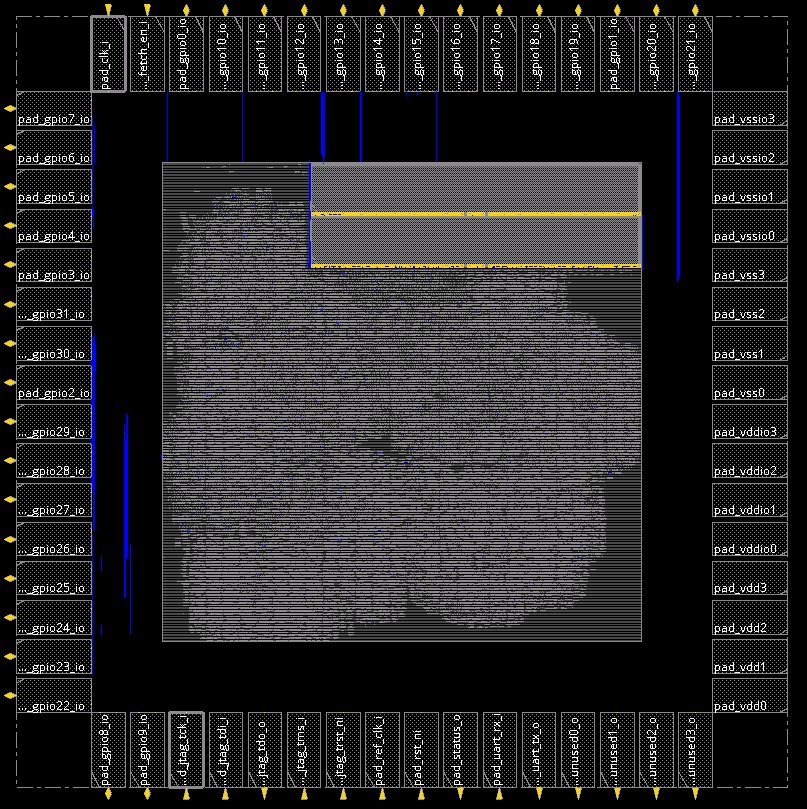
\includegraphics[width=0.45\textwidth]{routing_metal_1.png}
    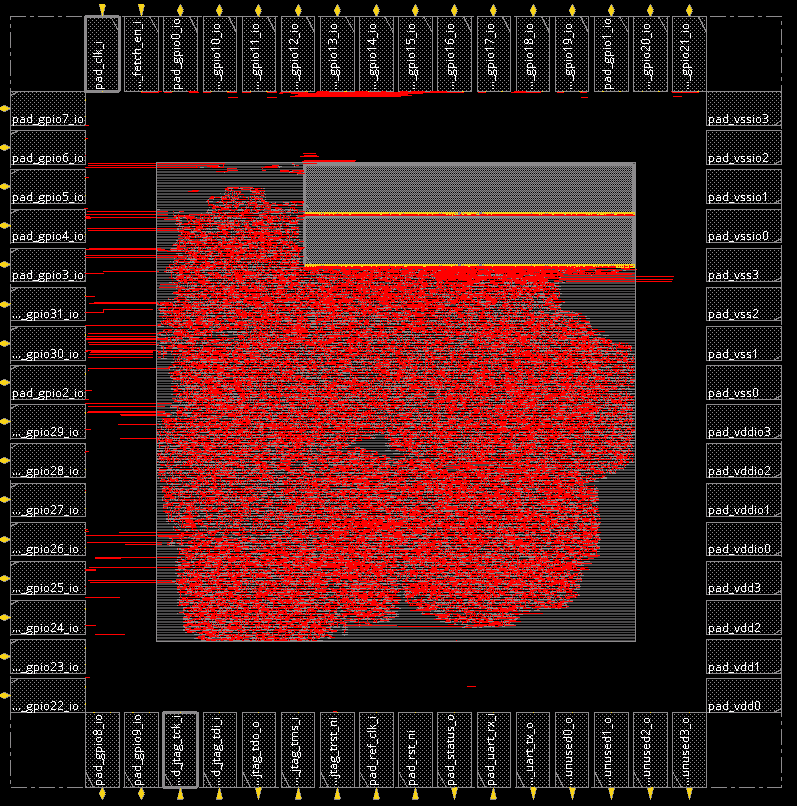
\includegraphics[width=0.45\textwidth]{routing_metal_2.png}
    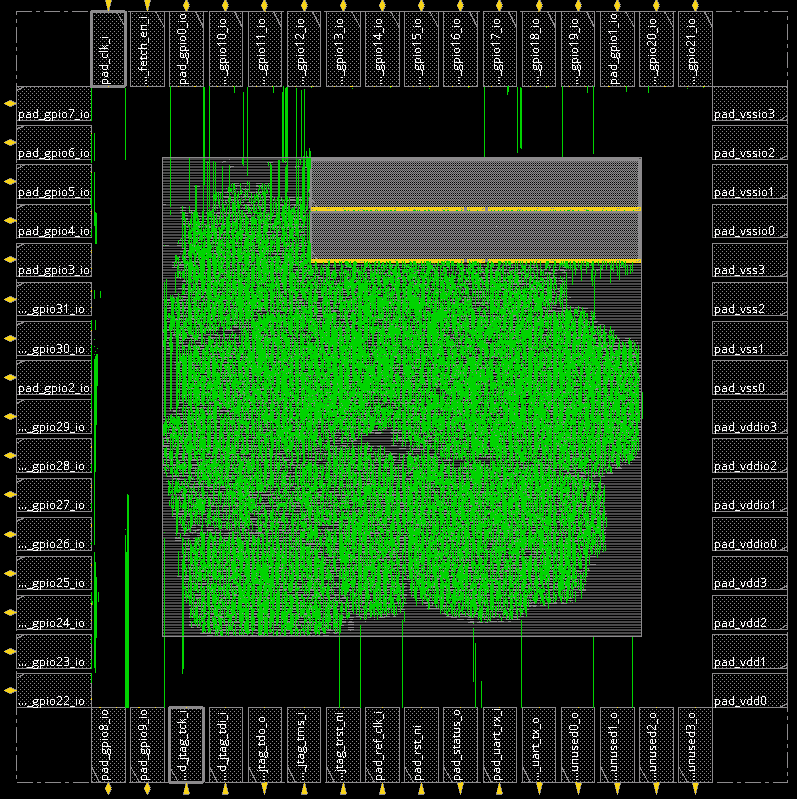
\includegraphics[width=0.45\textwidth]{routing_metal_3.png}
    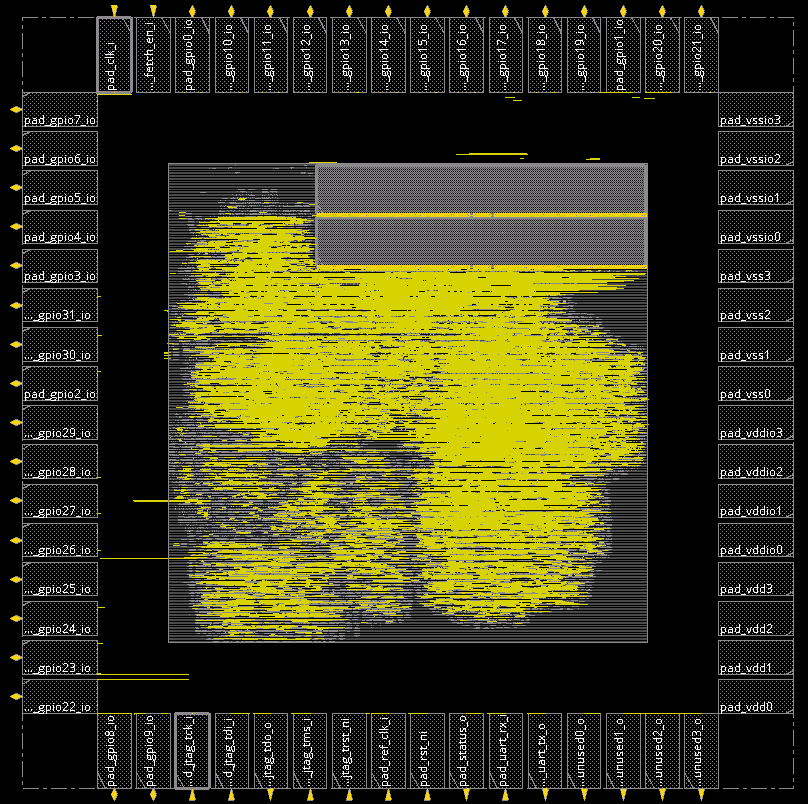
\includegraphics[width=0.45\textwidth]{routing_metal_4.png}
    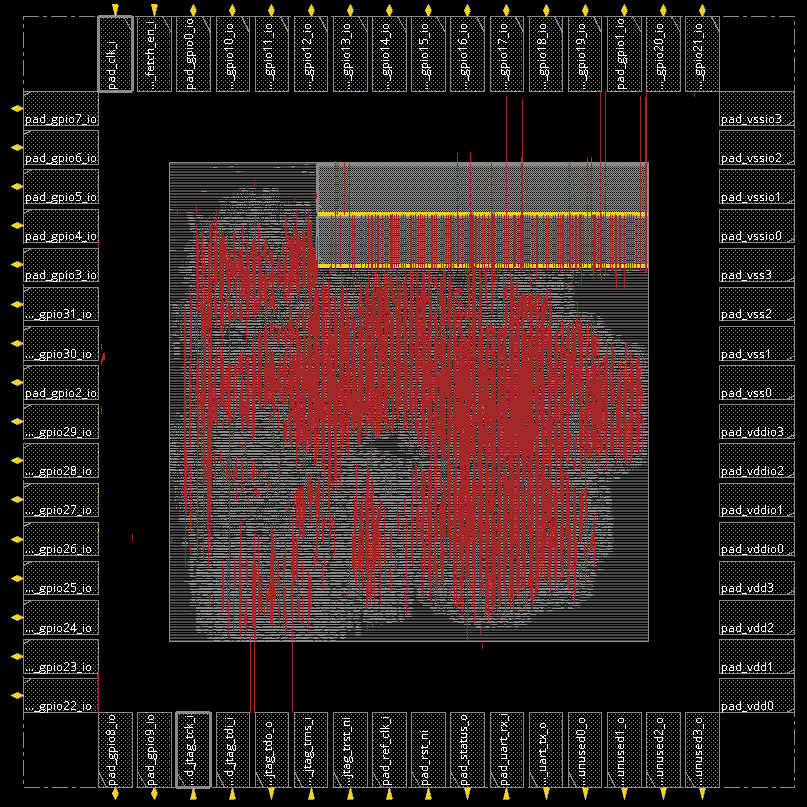
\includegraphics[width=0.45\textwidth]{routing_metal_5.png}
    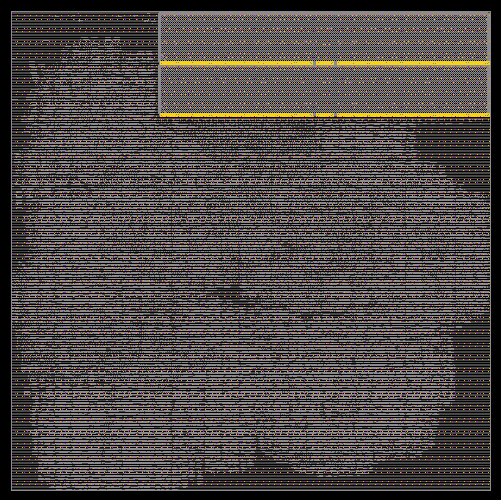
\includegraphics[width=0.45\textwidth]{via.png}
    \caption{Hình ảnh routing đi dây lần lượt từ M1 $\rightarrow$ M5 và Via}
\end{figure}

\begin{figure}[H]
    \centering
    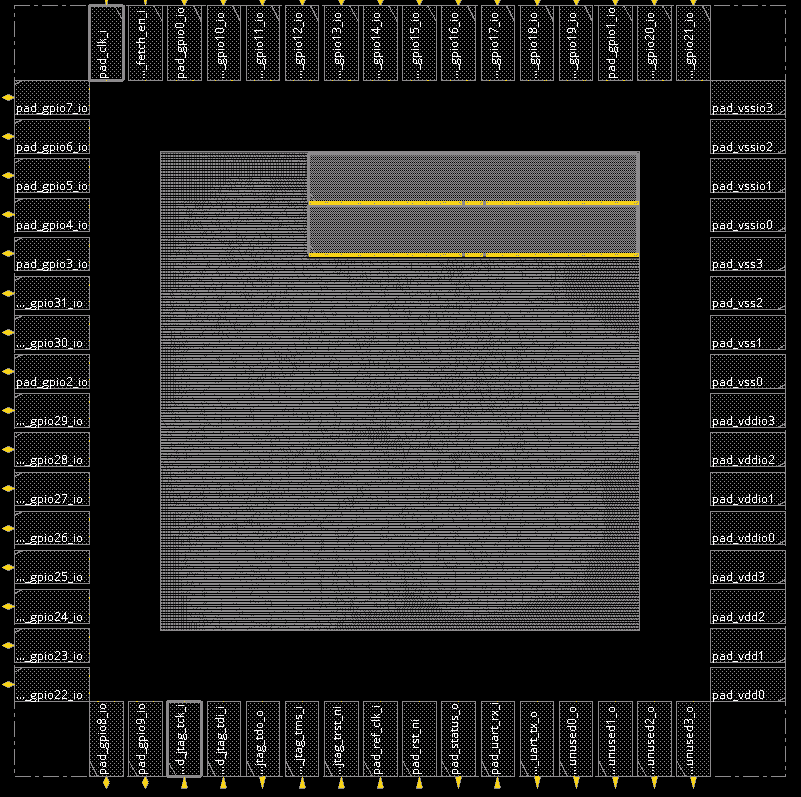
\includegraphics[width=0.48\textwidth]{fillercell_added.png}
    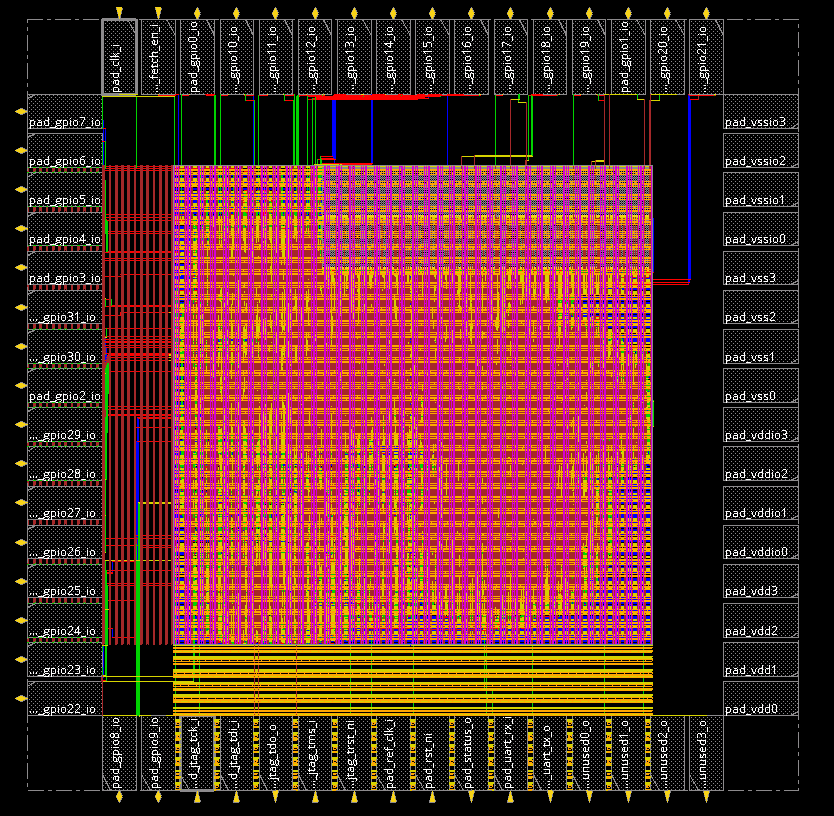
\includegraphics[width=0.48\textwidth]{full_chip.png}
    \caption{Chèn Filler Cells (trái) và Bố cục hoàn thiện toàn bộ chip (phải)}
\end{figure}

\end{document}
